\documentclass{beamer}

\usetheme{Szeged}
\usecolortheme{beaver}
\beamertemplatenavigationsymbolsempty

\definecolor{ao}{rgb}{0.0, 0.5, 0.0}

\usepackage{booktabs}
\usepackage{tikz}

\title{Distributional Gastronomics}
\author[Oberl\"ander and Bostan]{Jonathan Oberl\"ander and Laura Bostan}
\institute[Trento University]{Trento Universtity\\\vspace{1cm}
\includegraphics[scale=0.08]{pics/esslli.png}}
\date{}%August 10, 2015}

\addtobeamertemplate{frametitle}{}{%
    \begin{tikzpicture}[remember picture,overlay]
        \node[anchor=north east,yshift=-20.65pt] at (current page.north east) {
\includegraphics[height=0.8cm]{pics/esslli.png}};
\end{tikzpicture}}

\begin{document}

\maketitle %maybe

\section{Distributional Semantics}

\begin{frame}
    \frametitle{Formal Semantics}
    {\footnotesize [Frege et al.]}\\

    meaning of a sentence: (assigned) meanings of words and \textit{how they are combined}

    \vspace{0.3cm}

    \centering\includegraphics[scale=0.25]{pics/foo.png}
\end{frame}

\begin{frame}
    \frametitle{Distributional Semantics}
    {\footnotesize [Wittgenstein, Firth, ..., Landauer, Baroni, ...] }\\
    Distributional hypothesis: Similar words appear in similar contexts

    \vspace{0.5cm}

    % Less functional words, more content words

    %\centering\includegraphics[scale=0.6]{pics/dsbaroni.png}
    \centering

    {\tt
    \scalebox{0.7}{
        \begin{tabular}{rcl}
            \textcolor{blue}{Capital} to be as \textcolor{blue}{hot} as & \textcolor{red}{Barcelona} & as \textcolor{blue}{temperatures} soar\\
            \textcolor{blue}{sleep} on \textcolor{blue}{hot} \textcolor{blue}{nights} and & \textcolor{red}{Barcelona} & often has very \textcolor{blue}{hot}\\
            \textcolor{blue}{street} of the \textcolor{blue}{gothic} & \textcolor{red}{Barcelona} & and stumbled upon this\\
            the sweetest \textcolor{blue}{street} in & \textcolor{red}{Barcelona} & So, for those who \textcolor{blue}{love}\\
            about \textcolor{blue}{street} \textcolor{blue}{food} in & \textcolor{red}{Barcelona} & without mentioning the\\
    \end{tabular}
}
    }

    \pause

    \vspace{0.5cm}

    \begin{tabular}{rrrr}
        \toprule
        & \textcolor{blue}{hot} & \textcolor{blue}{street} & \cdots \\
        \midrule
        \textcolor{red}{Barcelona} & 22 & 30 & \cdots\\
        \textcolor{ao}{Trento} & 15 & 13 & \cdots\\
        \textcolor{orange}{desert} & 27 & 3 & \cdots\\
        \bottomrule
    \end{tabular}
\end{frame}

\begin{frame}
    \frametitle{Distributional Semantics: Word Relatedness}

    %\begin{columns}[onlytextwidth]
        %\begin{column}{0.6\textwidth}
        \centering
        \includegraphics[scale=0.4]{pics/barcelonetta.png}
        %\end{column}

        %\begin{column}{0.4\textwidth}
        %scaling,

        %dimensionality reduction
        %\end{column}
    %\end{columns}

    % "and additional stuff: weighting, dimensionality reduction, composing (?)
\end{frame}

\section{Distributional Gastronomics}

\begin{frame}
    \frametitle{Distributional Gastronomics}
    % \dots{}One day, we were hungry.
    \centering\includegraphics[scale=0.3]{pics/italy.jpg}

    \pause
    Distributional \textbf{gastronomical} hypothesis: Similar \textbf{ingredients} appear in similar contexts
\end{frame}

\begin{frame}
    \frametitle{Open Recipes}
    \centering\includegraphics[scale=0.5]{pics/openrecipes.png}
\end{frame}

\begin{frame}
    \frametitle{Open Recipes}

    {\tt

        \footnotesize{12 whole Dinner Rolls Or Small Sandwich Buns (I Used Whole Wheat)}

        \footnotesize{1 pound Thinly Shaved Roast Beef Or Ham (or Both!)}

        \footnotesize{10 ounces carrots, shredded on a box grater or sliced whisper thin on a mandolin}

        \footnotesize{optional: whole pomegranate seeds or fresh/dried rose petals, a bit of bee pollen}
    }\pause

    \vspace{0.5cm}
    \centering
    \scalebox{0.7}{
    \begin{tabular}{lr}
        \toprule
        \textbf{Number of recipes} & 172893\\
        \textbf{Number of ingredients (tokens in corpus)} & 1689892\\
        \textbf{Number of ingredients (types in corpus)} & 412858\\
        \textbf{Number of ingredients (types after unifying)} & 6514\\
        \bottomrule
    \end{tabular}
    }
    %Co-occurences of ingredients in Open Recipes
    % ingredient extraction, cleaning
    % count co-occurrences of ingredients

\end{frame}

\begin{frame}
    \frametitle{Pipeline}
    Creating the \textbf{Ingredients} space:
    \vspace{0.2cm}

    \begin{center}

    Corpus

    $\downarrow$

    Cleaning and ingredient unification

    $\downarrow$

    Co-occurrence counts

    $\downarrow$

    Re-Weighting (PPMI)

    $\downarrow$

    Scaling (SVD; 20 dimensions)

\end{center}

\end{frame}

\begin{frame}
    \frametitle{\textbf{Ingredients}: 2D projection of top ingredients}

    \centering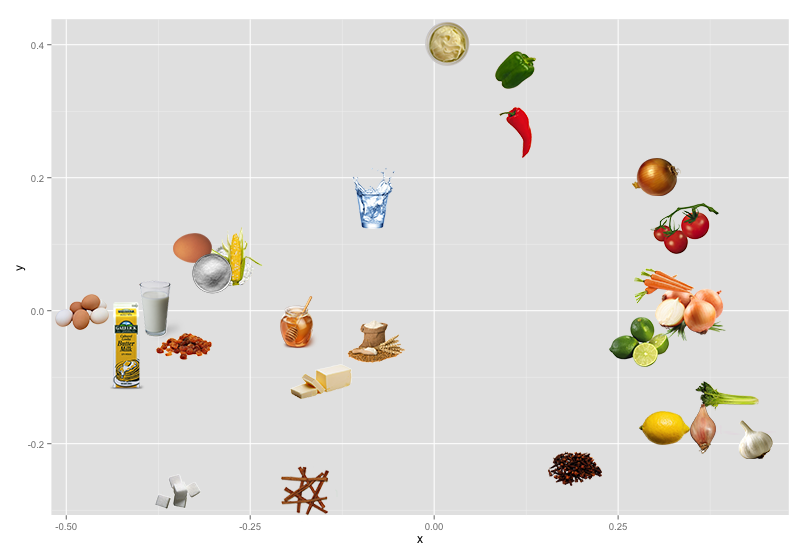
\includegraphics[scale=0.35]{pics/ingredipic.png}
\end{frame}

\begin{frame}
    \frametitle{\textbf{Ingredients}: Top neighbors of ``grapes''}
    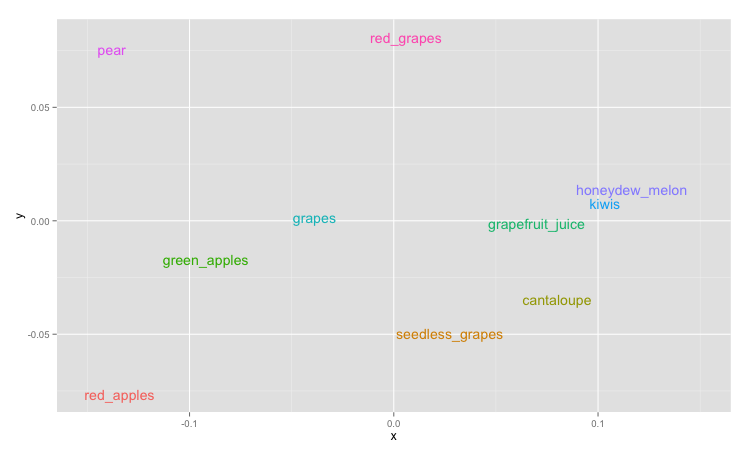
\includegraphics[scale=0.4]{pics/grapes_final.png}
\end{frame}

\begin{frame}
    \frametitle{Recipe spaces}

    \textbf{BasicRecipes}: recipes co-occurs with all of its ingredients

    \vspace{0.2cm}

    \textbf{ComposedRecipes}: recipe is the sum of the vectors of its ingredients

    \vspace{0.2cm}

    \begin{center}
        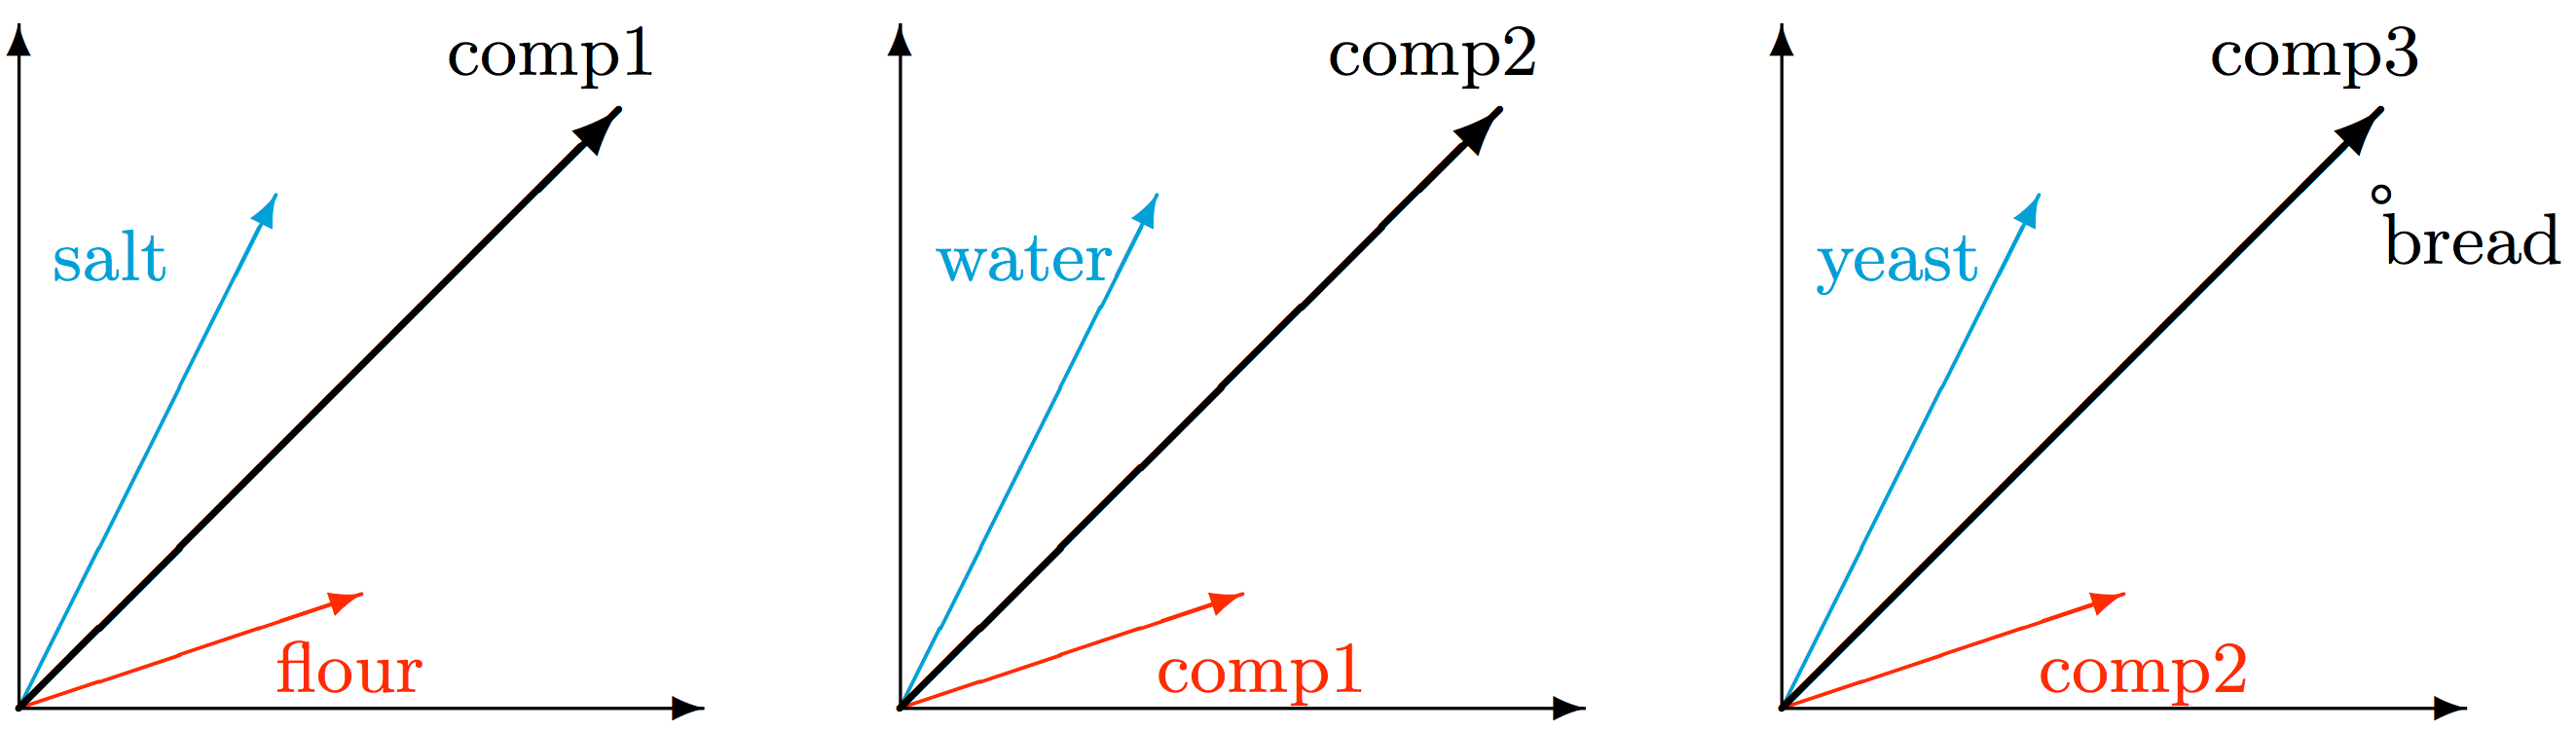
\includegraphics[scale=0.2]{pics/figure2.png}
    \end{center}
\end{frame}

\begin{frame}
    \frametitle{Applications}

    \includegraphics[width=\textwidth]{pics/neighbors.png}

    \includegraphics[width=\textwidth]{pics/makeme.png}

\end{frame}

\begin{frame}
    \frametitle{Credits}

    \scalebox{0.8}{
    \begin{tabular}{rl}
        \textbf{Questions?} & Come and see our poster.\\
        \textbf{Ideas?} & Come and see our poster.\\
        \textbf{Criticism?} & Come and see our poster.\\
        \textbf{Want to experiment with our scripts?} & Come and see our poster.\\
        \textbf{Want to plot the neighbors of chocolate?} & Come and see our poster.\\
    \end{tabular}}

    \vspace{2cm}

    \footnotesize{Formal Semantics picture stolen from: Anca Dinu}
\end{frame}

\begin{frame}
    \frametitle{Fuck Grapefruit}
    \centering

    \includegraphics[width=\textwidth,height=0.6\textheight,keepaspectratio]{pics/fuckgrapefruit.png}

    \textsmall{Coconuts are so far down to the left they couldn't be fit on the chart.  Ever spent half an hour trying to open a coconut with a rock? Fuck coconuts.}

    \footnotesize{(https://xkcd.com/388)}

\end{frame}

\end{document}
